\section{World-machine relationship}

The machine signifies the portion of the system to be developed, while the world denotes the segment of the real-world influenced by the machine. 
It is crucial to note that the machine's purpose always resides within the context of the world.

Requirements engineering is primarily concerned with phenomena occurring in the world, rather than those confined to the machine itself. 
In essence, requirements models serve as representations of real-world phenomena.
 
Certain phenomena are shared between the world and the machine. 
These shared phenomena fall into two categories:
\begin{itemize}
    \item Phenomena controlled by the world and observed by the machine.
    \item Phenomena controlled by the machine and observed by the world.
\end{itemize}
\begin{figure}[H]
    \centering
    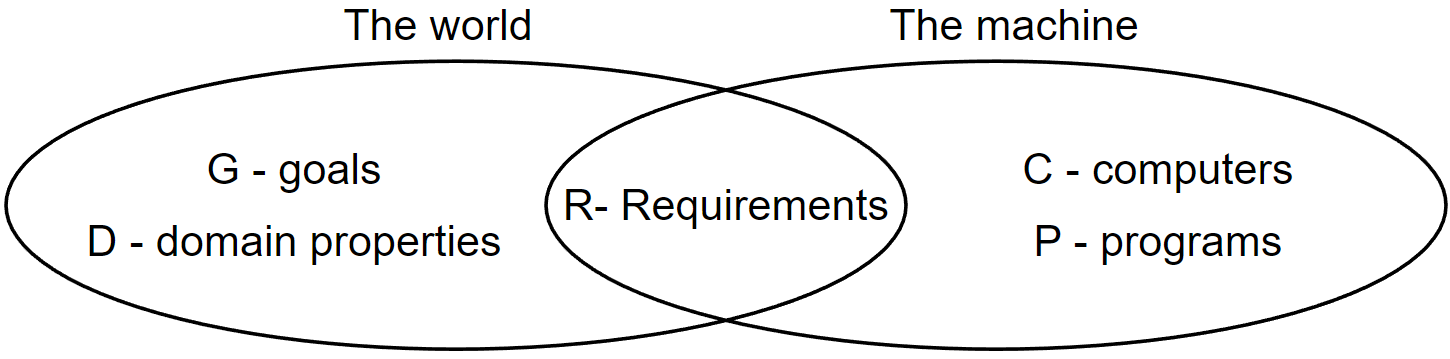
\includegraphics[width=0.75\linewidth]{images/worldmachine.png}
    \caption{Goals, domain assumptions, and requirements}
\end{figure}
Goals are declarative statements formulated in terms of real-world phenomena, which may or may not be shared.
Domain properties and assumptions, on the other hand, are descriptive statements presumed to be valid in the world. 
Requirements, as prescriptive assertions, are expressed in terms of shared phenomena.
  
The completeness of requirements, denoted as $R$, is achieved if:
\begin{itemize}
    \item $R$ guarantees the satisfaction of goals $G$ within the context of domain properties $D$, expressed as $R\land D \models G$.
    \item $G$ comprehensively capture all the needs of stakeholders.
    \item $D$ accurately represent valid properties and assumptions about the world.
\end{itemize}